\section{Exercícios}

\begin{exercise}
A escala $N$ de temperaturas foi feita com base nas temperaturas máxima e mínima em Nova Iguaçu. 
A correspondência com a escala Celsius é a seguinte:
%
\begin{center}
\begin{tabular}{|r|r|}
  \hline
  \tdeg N & \tdeg C \\ \hline
  0 & 18 \\ \hline
  100 & 43 \\ \hline
\end{tabular}
\end{center}
Modele o problema com funções afins que transformem a temperatura em
\tdeg N em \tdeg C e vice-versa. Qual a relação entre essas duas funções? Em
que temperatura ferve a água na escala $N$?
\end{exercise}

\begin{exercise}
\label{exer:determinicidade-funcao-afim}
Mostre que uma função afim $f: \R \to \R$ fica inteiramente
determinada quando conhecemos $f(x_1)$ e $f(x_2)$ para $x_1 \neq
x_2$.
\end{exercise}

\begin{exercise}
Pessoas apressadas podem diminuir o tempo gasto em uma escada
rolante subindo alguns degraus da escada no percurso. Para uma certa
escada, observa-se que uma pessoa gasta 30 s na escada quando
sobe 5 degraus e 20 s quando sobe 10 degraus. Quantos são os
degraus da escada e qual o tempo gasto no percurso?
\end{exercise}

\begin{exercise}\label{exercicio:juros-simples}
  Uma aplicação financeira rende a \emph{juros simples} quando os juros são calculados somente sobre a aplicação inicial durante todo o período de tempo.

  Edson faz uma aplicação que rende juros $j>0$ em um mês. Ou seja, se ele investiu um capital inicial $c_0$, então ao fim de 1 mês, Edson poderia resgatar $c = c_0(1+j)$. Caso a aplicação renda juros simples, defina uma função afim que calcule o capital $c_s$ em função do tempo $t$ (em meses) da aplicação.
\end{exercise}

\begin{exercise}
    Dada as PAs $\paren{a_1, a_2, \dots, a_n, \dots}$, de razão não
nula, e $\paren{b_1, b_2, \dots, b_n, \dots}$, mostre que existe
uma, e somente uma, função afim $f: \R \to \R$ tal que $f(a_1) =
b_1$, $f(a_2) = b_2$, \dots , $f(a_n) = b_n$, \dots
\end{exercise}

\begin{exercise}
  Os termos $a_1, a_2, \dots, a_n, \dots$ de uma PA são os valores
  $f(1), f(2), \dots, f(n), \dots$ de uma função afim, tal que $f(n)
  >0$ para todo $n \in \N^\ast$.

  \begin{enumerate}[a)]
    \item Mostre que cada $a_i$ é igual à área de um trapézio
    delimitado pelo gráfico de $f$, pelo eixo $x$ e pelas retas
    verticais de equações $x=i - \frac 1 2 $ e $x = i + \frac 1 2$.
    
    \begin{figure}[H]
      \centering
      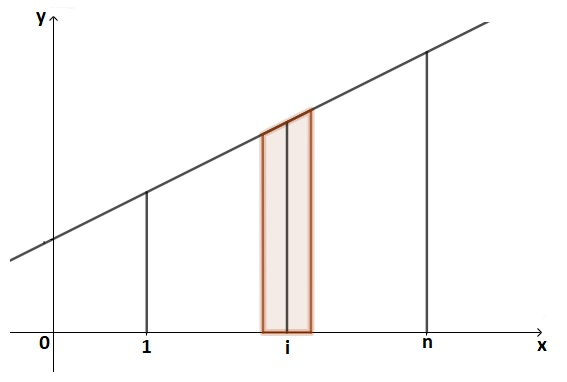
\includegraphics[height=0.3\paperheight]{\imgdirfromsection/exercicio-trapezio.jpg}
      \label{fig:exercicio-trapezio}
    \end{figure}

    \item Mostre, por indução, que a soma $S_n = a_1+a_2+ \dots + a_n$ é igual à
    área do trapézio delimitado pelo gráfico de $f$, pelo eixo $x$ e
    pelas retas verticais $x= \frac 1 2$ e $x = n + \frac 1 2 $.
    \item Conclua, a partir da área do trapézio, que $S_n = \frac{a_1+a_n} 2 n$.
  \end{enumerate}
\end{exercise}

\begin{exercise}
    Para cada uma das funções quadráticas abaixo, escreva-a na forma
$f(x)=a(x-m)^2+k$. A seguir, calcule suas raízes (se existirem), o
eixo de simetria de seu gráfico e seu valor mínimo e máximo.
%
\begin{enumerate}[a)]
  \item $f(x) = x^2 -8x +23$;
  \item $f(x) = 8x - 2x^2$;
  \item $f(x) = 2x^2 - 16x +46$.
\end{enumerate}
\end{exercise}

\begin{exercise}
  Considere a função real $f : \R \to \R$ tal que $f(x) = x^2 -7x +12$.
  \begin{enumerate}[a)]
    \item Calcule as raízes de $f$ e qual $x_0 \pertence \R$ é mínimo absoluto de $f$;
    \item Mostre que $f$ é monótona (crescente ou decrescente) no intervalo $\left( - \infty , x_0 \right] = \conjunto{x \pertence \R; x \leq x_0 }$;
    \item Utilize os itens anteriores e o exercício \ref{exercicio:polinomio} do Capítulo \ref{cap:principio-da-inducao-finita} para concluir que $n^2 - 7n +12 \geq 0$ para todo $n \pertence \Z$.
  \end{enumerate}
\end{exercise}

\begin{exercise}
    Encontre os valores mínimo e máximo assumidos pela função $f(x)
= x^2 -4x +3$ em cada um dos intervalos abaixo:
\begin{enumerate}[a)]
  \item $\bracket{1, 4}$;
  \item $\bracket{6, 10}$.
\end{enumerate}
\emph{Dica:} Esboce o gráfico de $f(x)$ nos intervalos indicados
para visualizar melhor os valores mínimo e máximo assumidos pela
função.
\end{exercise}

\begin{exercise}
    Os alunos de uma turma fizeram uma coleta para juntar 405 reais,
custo de uma excursão. Todos contribuíram igualmente. Na última
hora, dois alunos desistiram. Com isso, a parte de cada um sofreu um
aumento de um real e vinte centavos. Quantos alunos tem a turma?
\end{exercise}

\begin{exercise}
  Considere o retângulo $ABCD$ inscrito em uma circunferência de raio $r = 2$, conforme ilustra a figura abaixo.
  \begin{figure}[H]
    \centering
    \label{fig:exercicio-retang_inscrito}
    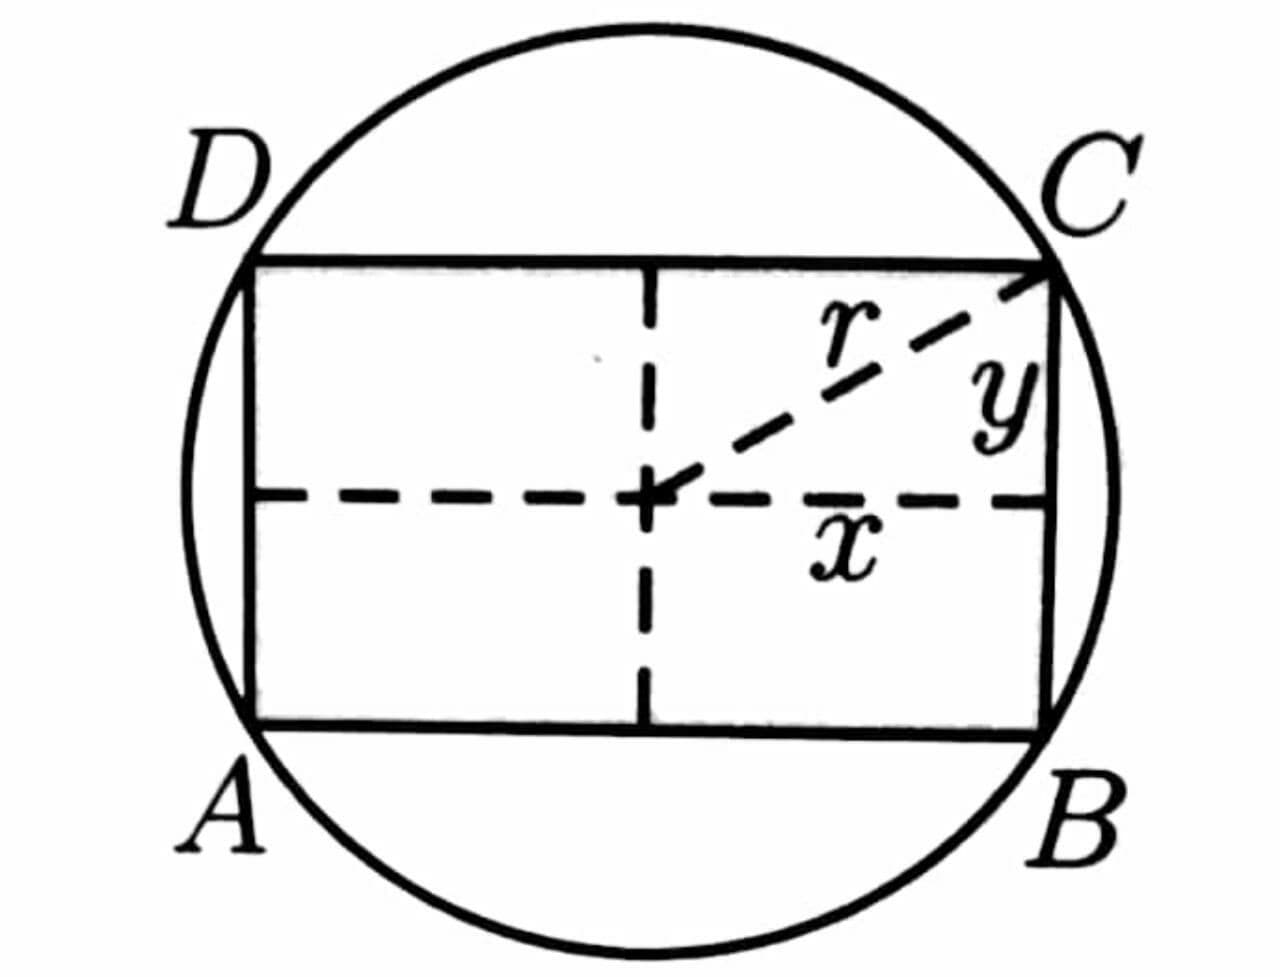
\includegraphics[width=7cm]{\imgdirfromsection/exercicio-retang_inscrito.jpg}
    \caption{Retângulo inscrito em circunferência.}
  \end{figure}
  \begin{enumerate}[a)]
      \item Qual a equação que determina $y$ em função de $x$ e $r$?
      \item Defina uma função polinomial, incluindo domínio e contradomínio, que receba o valor de $x$ e retorne a área do retângulo.
      \item Quais os valores de $x$ e $y$ tais que a área do retângulo seja máxima? 
      \begin{hint}
        Obtenha o valor de $x$ que maximiza a área ao quadrado, pois é o mesmo que maximiza a área, já que são valores positivos. Ao encontrar um polinômio de grau 4, faça $z=x^2$ para calcular onde ocorre máximo do novo polinômio, agora de grau 2.
      \end{hint} 
  \end{enumerate}
\end{exercise}

\begin{exercise}
  Considere a função polinomial $p(x)=x^2-2$.
  \begin{enumerate}[a)]
    \item Usando o Teorema de raízes racionais prove que $p(x)$ não possui raízes racionais;
    \item Mostre que $\raiz{2}$ é raiz de $p(x)$;
    \item Conclua que $\raiz{2}$ é irracional.
  \end{enumerate}
\end{exercise}

\begin{exercise}
  Considere a função polinomial $p(x)=x^2-q$, onde $q \pertence \N^\ast$ é um número primo.
  \begin{enumerate}[a)]
    \item Usando o Teorema de raízes racionais prove que $p(x)$ não possui raízes racionais;
    \item Mostre que $\raiz{q}$ é raiz de $p(x)$;
    \item Conclua que $\raiz{q}$ é irracional.
\end{enumerate}
\end{exercise}

\begin{exercise}
    Determine o polinômio $p(x)$ de menor grau possível tal que
$p(1) = 2$, $p(2)=1$, $p(3) = 4$ e $p(4) = 3$.
\end{exercise}

\begin{exercise}
Mostre que, se $n$ é um número par, então o polinômio $p(x) =
x^n + x^{n-1} + \dots + x+1$ não possui raiz real.

\noindent \emph{Dica: } Note que, para $x \neq 1$, $p(x) =
\frac{x^{n+1}-1}{x-1}$. Proceda supondo, por contradição, que existe
$a \neq 1$ raiz de $p(x)$.
\end{exercise}